\begin{figure}[htbp]
    \begin{subfigure}{0.49\textwidth}
    \centering
      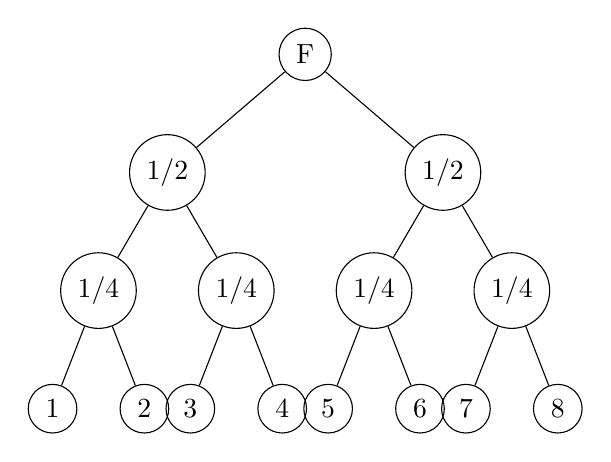
\begin{tikzpicture}[
        every node/.style = {circle, draw, minimum size=0.6cm},
        level/.style = {sibling distance=3.5cm/#1}
    ]
    \node {F}
        child {node {1/2}
            child {node {1/4}
                child {node {1}}
                child {node {2}}
            }
            child {node {1/4}
                child {node {3}}
                child {node {4}}
            }
        }
        child {node {1/2}
            child {node {1/4}
                child {node {5}}
                child {node {6}}
            }
            child {node {1/4}
                child {node {7}}
                child {node {8}}
            }
        };
    \end{tikzpicture}
    \caption{Arbre complet}
    \label{fig:arbre_complet}
    \end{subfigure}%
    \hfill
    \begin{subfigure}{0.49\textwidth}
    \centering
      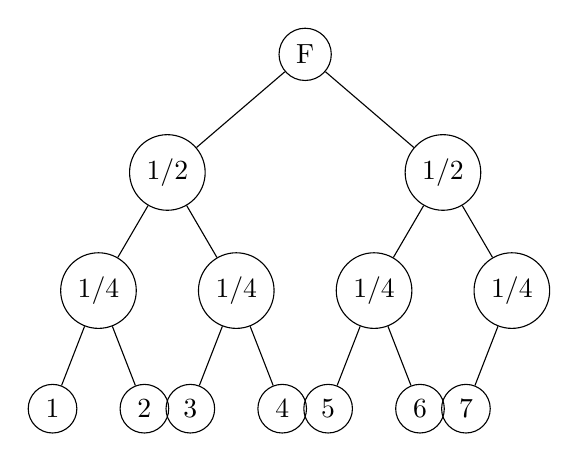
\begin{tikzpicture}[
        every node/.style = {circle, draw, minimum size=0.6cm},
        level/.style = {sibling distance=3.5cm/#1}
    ]
    \node {F}
        child {node {1/2}
            child {node {1/4}
                child {node {1}}
                child {node {2}}
            }
            child {node {1/4}
                child {node {3}}
                child {node {4}}
            }
        }
        child {node {1/2}
            child {node {1/4}
                child {node {5}}
                child {node {6}}
            }
            child {node {1/4}
                child {node {7}}
                child[missing]
            }
        };
    \end{tikzpicture}
    \caption{Arbre incomplet}
    \label{fig:arbre_incomplet}
    \end{subfigure}
\end{figure}
